\chapter{Integración del sistema en una API}\label{chap:api}

Se ha visto que es una regla general en los trabajos de fin de estudios (no únicamente de UNIR, sino en general) orientados al Data Science y el análisis de datos la no creación de un entorno que podría denominarse productivo. Muchos de estos trabajos se centrar en realizar un análisis de los datos e implementar modelos predictivos, pero siempre en un entorno que podría considerarse ``de laboratorio''. Sin embargo, creemos que un TFE además de ser una forma de finalizar unos estudios, debería ser el inicio de aquello que viene después de ellos; el mundo real.\\

En este caso, el tema del TFE son los sistemas de recomendación de contenido. En este trabajo se ha revisado en primer lugar su necesidad en el entorno digital actual, en el que existen plataformas con muy variado contenido y usuarios que tienen que ser capaces de navegar por él. Además, se ha realizado una revisión teórica de los sistemas de recomendación, habiéndose explicado los principales tipos y sus aplicaciones. El caso de uso concreto que se ha llevado a cabo en este TFE ha sido relacionado con las películas. Se ha realizado un flujo completo de adquisición y preparación de los datos, a partir de diferentes datasets y se ha construido con ellos un sistema de recomendación. El sistema utiliza las palabras clave de cada película, el director, los actores, el año de lanzamiento y la popularidad de la película, para recomendar a un usuario películas dada una de referencia.\\

Como se ha explicado en el primer párrafo, consideramos que un TFE de desarrollo de software debería estar orientado a una implementación en el mundo real, en el que usuarios reales pudieran hacer uso del mismo. Este es un paso que suele dejarse indicado en los próximos pasos, no siendo así en este proyecto. Se implementará el sistema de recomendación en una REST API en Python utilizando la librería Flask y esta API será llamada por un bot de Telegram para responder a los usuarios.

\section{Telegram}

Telegram es una compañía de mensajería instantánea en la nube. Dispone de clientes para la mayoría de plataformas (Android, iOS, Windows Phone, macOS, linux...) y los usuarios pueden intercambiar mensajes, fotos, videos, audio, stickers o archivos de cualquier tipo. Además, la parte del cliente de Telegram es software libre (no así la parte de back-end), aunque en ocasiones la publicación no es inmediata. Como puede deducirse, Telegram es una compañía competidora de Whatsapp, aunque contiene características muy diferentes y atractivas.\\
\begin{figure}[H]
    \centering
    \captionsetup{width=7cm}
    
\includegraphics[width=5cm]{contenido/imagenes/Telegram-logo.jpg}
    \caption{Logo de la aplicación Telegram. Fuente: Wikipedia \cite{wiki:telegramImage}}
\end{figure}
Entre las innumerables características de Telegram, en este proyecto la de mayor importancia es la posibilidad de crear bots. Los bots de Telegram son aplicaciones de terceros que corren dentro de Telegram. Los usuarios pueden interactuar con los bots enviándoles mensajes y comandos. Entre las posibilidades de un bot se encuentran:
\begin{itemize}
    \item Obtener notificaciones personalizadas y noticias. Un bot puede actuar como un periódico, enviando contenido relevante para cada usuario de forma instantánea.
    \item Integrarse con otros servicios como GMail, GitHub o YouTube, permitiendo al usuario recibir, por ejemplo, notificaciones sobre cambios en sus repositorios.
    \item Aceptar pagos de usuarios de Telegram, gracias a la posibilidad de un bot de ofrecer servicios de pago.
    \item Creación de herramientas personalizadas, como alertas, previsiones meteorológicas, control domótico de la casa...
    \item Creación de juegos tanto de un jugador como para varios jugadores.
\end{itemize}

En resumen, existen bots para realizar prácticamente cualquier tarea, y en caso de que no exista, es posible crearlo si se dispone de las herramientas y los conocimientos adecuados; además de forma gratuita.\\

Los bots se distinguen de los humanos por su nombre (debe contener ``bot''), por no necesitar un teléfono para crear la cuenta y por no poder iniciar conversaciones con usuarios. Es el usuario quien debe iniciar una conversación con ellos.\\

En este caso particular, se utilizara Telegram como interfaz entre el usuario y el sistema de recomendación, tanto por sus cualidades como por su relativa facilidad de uso.\\

Para crear el bot, simplemente hay que iniciar una conversación con el bot \textit{@botfather} y enviar el comando \textit{$\backslash$newbot}, nos pedirá un nombre para el bot y un nombre de usuario, que tendrá que terminar en ``bot''. Una vez realizados estos pasos, se proporcionará el token que permite realizar modificaciones en el bot e interactuar a través de la API de Telegram. En la \autoref{fig:botfather} se muestra el proceso de creación del bot.

\begin{figure}[H]
    \centering
    \captionsetup{width=8cm}
    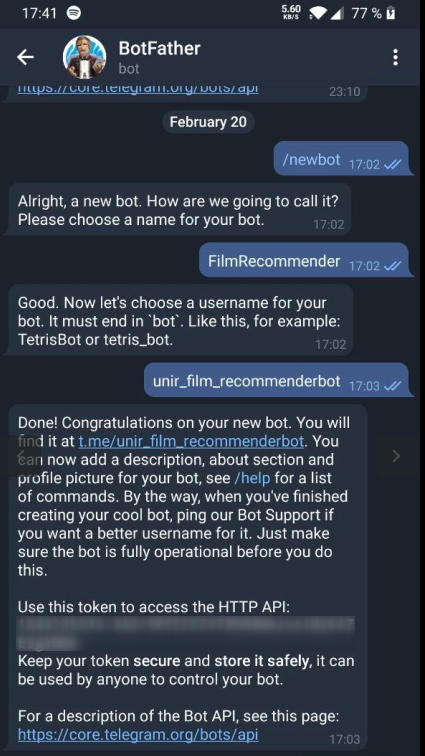
\includegraphics[width=6cm]{contenido/imagenes/botfather.png}
    \caption{Creación de un bot en Telegram mediante una conversación con el usuario \textit{@botfather}.}
    \label{fig:botfather}
\end{figure}


El funcionamiento del bot es el siguiente (puede obtenerse documentación más detallada en \cite{Telegram}):

\begin{enumerate}
    \item Se crea un webhook para que el bot envíe los mensajes que reciba a la URL que le proporcionemos, utilizando el siguiente método de la API: \url{https://api.telegram.org/bot<token>/setWebHook?url=<url_API>/telegram/}. De esta forma, cada vez que el bot reciba un mensaje, lo enviará a la URL de la API en formato JSON, para que la repuesta se procese.
    \item Se procesa el mensaje en la API creada (esta parte se detallará en la \autoref{sec:API}).
    \item Una vez la API ha procesado la petición del usuario y tiene la respuesta a enviar, se ejecuta la siguiente petición a la API de Telegram: \url{https://api.telegram.org/bot<token>/sendMessage?chat_id=<chat_id>&parse_mode=Markdown& text=<answer>}.
\end{enumerate}

Con estos simples pasos es posible crear un usuario de Telegram con el que cualquier usuario pueda interactuar, enviarle películas y obtener recomendaciones. Como se ha visto, la Telegram es un servicio con mucho potencial y relativamente sencillo y económico de implementar.

\section{Creación de la API en Python} \label{sec:API}

En la sección anterior se ha descrito de forma detallada el funcionamiento del chatbot desde el punto de vista de la API de Telegram, habiéndose explicado el funcionamiento de los bots en general y los pasos a seguir para crear un chatbot en esta plataforma. En esta sección se abordará el otro punto de vista, el de la API creada para implementar el sistema de recomendación.\\

Flask \cite{wiki:FlaskHelloWorld} es un micro framework web escrito en Python para crear aplicaciones web, es decir, páginas dinámicas, API, etc. Existen alternativas en Python como Django, que han sido descartados por ser demasiado complejos, en este caso se necesita crear una API relativamente sencilla. Es un framework rápido y sencillo.

\begin{figure}[H]
    \centering
    \captionsetup{width=7cm}
    \includesvg[width=9cm]{contenido/imagenes/flask}
    \caption{Logo del \textit{framework} Flask. Fuente: Wikipedia \cite{wiki:FlaskHelloWorld}}
\end{figure}

Mediante Flask se creará un servicio web que podrá ser llamado por el bot de Telegram, únicamente enviando a Telegram la URL del servicio Web y el token del bot. La API recibirá el mensaje, lo procesará y enviará al usuario la respuesta.\\

El ``hola mundo'' de Flask es el siguiente:

\begin{lstlisting}[language=Python, caption= {Aplicación Web básica creada con Flask. Se crea una API que devolverá la cadena de texto \textit{Hello world!} al ser invocada. Fuente: Wikipedia}]
from flask import Flask
app = Flask(__name__)

@app.route("/")
def hello():
    return "Hello world!"

if __name__ == "__main__":
    app.run(port = 8000)
\end{lstlisting}

Así, se tendría una aplicación web que en el puerto $8000$ devolvería ``Hello World''. Mediante los decoradores \texttt{@app.route()} se indica la ruta a través de la cual se entra a ese endpoint de la API.\\

La API se ejecutará en una Raspberry PI, debido a las ventajas que tiene en términos de coste frente a un servidor. Es de esperar que el servicio no tenga demasiadas solicitudes, por lo que tampoco tendrá problemas de volumen de peticiones. El problema es hacer que la API esté disponible a través de una URL. Para ello, dado que no se dispone de una IP estática ni de la posibilidad de abrir los puertos en el router, se utiliza el servicio \href{https://ngrok.com/}{Ngrok}. Ngrok es un servicio gratuito que publica un determinado puerto de localhost a través de una URL a través de un túnel.\\

Una vez explicado el funcionamiento, en el \autoref{lst:API}

\begin{lstlisting}[language=Python, label = {lst:API}, caption={Creación de la API del sistema de recomendación en Python usando Flask. En primer lugar se eliminan los posibles webhooks que existieran y se crea el nuevo con la URL a través de la cual pueda accederse a la API que estamos construyendo.}]
import requests
import time
import math
import os, json

from flask import Flask, request, json
from pyngrok import ngrok
from datetime import datetime
from configparser import ConfigParser
from datetime import timedelta
from recommendation import Recommendator
from utils import get_ngrok_url

# Lectura del fichero de configuración (Contiene el token)
config = ConfigParser()
config.read("telegram_config.ini")
telegram_token = config.get('mytokens', 'telegram')

# Creación del tunel seguro desde localhost
os.system('(./ngrok http 8000 &); exit')
time.sleep(2)

# Obtener la URL en la que está publicando el puerto 8000 ngrok
# (en el servicio gratuito es aleatoria)
url = get_ngrok_url()
url = url.replace('https://', '')
url = url.replace('http://', '')
print(url)


#Creación del webhook para que Telegram envíe los mensajes
deleteWebHook = 'https://api.telegram.org/bot' + telegram_token + '/deleteWebHook'
response_d = requests.get(deleteWebHook)
setWebHook = 'https://api.telegram.org/bot' + telegram_token + '/setWebHook?url=' + url+'/telegram/'
response = requests.get(setWebHook)
print(setWebHook)
print(response)
print(os.getcwd())

#Sistema de recomendación
recommendator = Recommendator()


app = Flask(__name__)
starting = math.floor(time.time())

@app.route('/')
def welcome():
    return 'Hola mundo'
@app.route('/telegram/', methods = ['POST', 'GET'])
def main ():
    
    # Mensaje recibido a través de TElegram y extracción de parámetros importantes
    recibido = dict(request.json)
    tiempo = recibido['message']['date']
    resta = tiempo-starting
    fecha_bien = datetime.fromtimestamp(starting).strftime("%A, %B %d, %Y %I:%M:%S")
    print(f'App started on {fecha_bien}')
    print(f"Message received {resta} seconds after starting.")
    if recibido["message"]["date"] > starting:
        # Caso en el que el mensaje se haya recibido con la aplicación operativa
        #(si no acumularía todos los mensajes y llegarían de repente)
        chat_id = str(recibido["message"]["chat"]['id'])
        usuario = recibido["message"]["chat"]["first_name"]
        mensaje = str(recibido["message"]["text"])
        print(usuario)
        print(recibido["message"]["text"])
        if mensaje != '/start':
            recommendation = recommendator.predict_from_string(mensaje)
            answer = recommendator.parse_response(recommendation)
        else:
            answer = """Welcome to the Film Recommendation Bot (built by Gonzalo Izaguirre).\n
            Just send us a title and we'll give you similar films."""
        
        send_text = 'https://api.telegram.org/bot' + telegram_token + '/sendMessage?chat_id=' + chat_id + '&parse_mode=Markdown&text=' + answer
        requests.get(send_text)
    return 'Hola Mundo'
if __name__ =='__main__':
    app.run(port = 8000)
\end{lstlisting}

En el \autoref{chap:creacion} se finalizó teniendo un sistema de recomendación que dado el id de una película, obtenía las películas recomendadas. Esto presenta un claro problema, ya que el usuario final no conocerá los ids, ya que son un identificador interno de la aplicación. Para obtener el id de una película a partir del mensaje del usuario se utiliza una estrategia similar a la seguida para saber si dos películas son secuelas o no. Utilizando lógica difusa y la distancia Levenshtein se compara la cadena de texto dada por el usuario con los títulos de las películas y se ordenan según su parecido. Si se supera un umbral determinado, se infiere que el título dado por el usuario se corresponde con el de mayor puntuación, y se buscan las recomendaciones utilizando ese id.

\begin{lstlisting}[language=Python, label = {lst:API}, caption= {Búsqueda del id de la película dada por el usuario. Estas funciones implementan la búsqueda de la película más parecida dentro de un umbral.}]
    @staticmethod
    def fuzzing(series_element, string):
        """Dadas dos cadenas de texto calcula la similaridad entre ambas. Se usa para cuando el usuario
        da como entrada una cadena de textopoder buscar la película a la que se refiere.
        Args:
            series_element (str): Cadena de texto 1
            string (str): Cadena de texto 2
        Returns:
            int: Similaridad entre las cadenas de texto
        """
        try:
            mark = 2/(1/fuzz.token_set_ratio(series_element.lower(), string.lower()) + 1/fuzz.ratio(series_element.lower(), string.lower()))
            return mark if mark > 60 else 0
        except:
            return 0

    def string_to_id(self, df, string):
        """Dada una cadena de texto se obtiene el id de la película que más se parece. Para ello se compara
        la cadena de texto con los títulos de las películas.
        Args:
            df (pd.DataFrame): DataFrame de películas
            string (str): Cadena de texto dada por el usuario.
        
        Returns:
            int: Id de la película encontrada.
        """
        df_2 = df.copy(deep = True)
        df_2["mark"] = df_2["movie_title"].apply(self.fuzzing , args = (string,))
        df_2.sort_values(by = ["mark", "title_year"], ascending = [False, True], inplace = True)
        #print("Parecido de la película introducida: ", df_2.iloc[0,-1])
        return df_2.index.values[0] if df_2.iloc[0,-1] > 60 else None
\end{lstlisting}

\section{Conversaciones de ejemplo}

En la \autoref{fig:TelegramResults} se muestran algunos ejemplos de conversaciones del chatbot de Telegram en las que el usuario aporta el título de una Película, y de una forma relativamente rápida ($\sim 10\ s$) el chatbot da las recomendaciones.\\


\begin{figure}[H]
\begin{subfigure}{.5\textwidth}
  \centering
  
\includegraphics[width=.9\linewidth]{contenido/imagenes/sc1.png}
  \caption{Recomendaciones para El señor de los anillos.}
  \label{fig:sc1}
\end{subfigure}%
\begin{subfigure}{.5\textwidth}
  \centering
  
\includegraphics[width=.9\linewidth]{contenido/imagenes/sc2.png}
  \caption{Recomendaciónes para Eragon}
  \label{fig:sc2}
\end{subfigure}
\\
\begin{subfigure}{.5\textwidth}
  \centering
  
\includegraphics[width=.9\linewidth]{contenido/imagenes/sc3.png}
  \caption{Recomendaciones para El señor de los anillos.}
  \label{fig:sc3}
\end{subfigure}%
\begin{subfigure}{.5\textwidth}
  \centering
  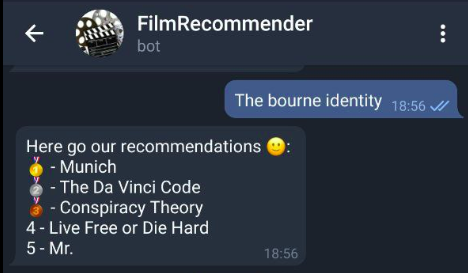
\includegraphics[width=.9\linewidth]{contenido/imagenes/sc4.png}
  \caption{Recomendación para El caso Bourne}
  \label{fig:sc4}
\end{subfigure}
\caption{Ejemplos de recomendaciones de películas dadas por el chatbot de Telegram. Le damos el título de una película y nos devuelve 5 recomendaciones ordenadas.}
\label{fig:TelegramResults}
\end{figure}

En este tipo de proyectos, resulta complicado evaluar los resultados. La calidad de las recomendaciones son algo bastante subjetivo, por lo que resulta complicado establecer una métrica de desempeño. Sin embargo, puede verse que las recomendaciones realizadas son relativamente acertadas, puesto que la temática y el género de las películas recomendadas es similar al de la dada.\\

\section{Código utilizado}

A lo largo del proyecto se ha ido adjuntando el código utilizado para cada una de las tareas, ya que creemos que resulta interesante conocer la estrategia seguida para tarea. Sin embargo, lo que se ha adjuntado son piezas de un Jupyter Notebook que genera el sistema de recomendación de forma interactiva (\autoref{app:notebook}. El código real se encuentra organizado en diferentes clases (preprocesado, imputación, recomendador, API...) para tener una estructura más organizada. El código puede consultarse en el repositorio de GitHub \url{https://github.com/gontxomde/RecommendationEngine} con una pequeña guía de despliegue y uso.\\

De la misma forma, a lo largo del proyecto, se han incluido en las funciones los denominados docstrings, que son formas estándar de definir el uso y los argumentos de una función en Python. La finalidad del uso de estos docstrings, además de hacer el código legible, es posibilitar el uso de Sphinx. Sphinx es un software que permite generar la documentación del código de forma automática, generando un documento html o latex fácilmente consultable. Además de en el repositorio antes mencionado, la documentación de la librería creada en este proyecto puede consultarse en el repositorio anteriormente mencionado.\\

Esperamos que esta forma de proceder a lo largo de la memoria haya facilitado la comprensión de los pasos seguidos para la creación del sistema de recomendación.


